%%%%%%%%%%%%%%%%%%%%%%%%%%%%%%%%%%%%%%%%%%%%%%%%%%%%%%%%%%%%%%%%
\begin{frame}
  \frametitle{Examples of a binary classification}
  \framesubtitle{The dataset $\dataset$}
\begin{displaymath}
\dataset = \left( 
{\color{green}
  \begin{array}{cccccccc}
    {\color{black} x_1=} &17 &12 &13 &15 &15 &20 &20\\
    {\color{black} x_2=} &10 &12 &14 &15 &20 &15 &20\\
    {\color{black} \class =} &1 &1 &1 &1 &1 &1 &1\\
    
  \end{array} 
}
\right.
\left.
{\color{red}
  \begin{array}{ccccccc}
4& 7.5& 10& 11& 5& 5& 6\\
8 &5 &0 &5 &0 &10& 6\\
0 &0 &0 &0 &0 &0 &0\\
  \end{array} 
}
\right)
\end{displaymath}
  \begin{center}
\only<1>{   \includegraphics[width=0.7\textwidth]{./figs/student_data.pdf}}
\only<2>{    \includegraphics[width=0.7\textwidth]{./figs/student_data_classes.pdf}}
  \end{center}
\end{frame}


%%%%%%%%%%%%%%%%%%%%%%%%%%%%%%%%%%%%%%%%%%%%%%%%%%%%%%%%%%%%%%%%
\begin{frame}
  \frametitle{Example of binary classification}
  \begin{block}{Goal: }
    \begin{itemize}
    \item Predict whether a candidate is hired ($\class = 1$) or not
      ($\class=0$) 
    \item knowing his results $\x$
    \item a candidate = 2 grades $\rightarrow \x = (x_1, x_2)$
    \end{itemize}
  \end{block}
  \begin{block}{The simplest model}
    \begin{align*}
      \class = 1 &\textrm{ if } w_1 x_1 + w_2 x_2 > \alpha \textrm{ otherwise } \class=0\\
      \class = 1 &\textrm{ if } w_0 + w_1 x_1 + w_2 x_2 > 0 \textrm{ otherwise }\class=0\\
      \class = 1 &\textrm{ if } w_0 + \scal{\vct{w}}{\x} > 0 \textrm{ otherwise }\class=0
    \end{align*}
    \end{block}
    \begin{block}{Learning}
      \begin{itemize}
      \item Find $\params =  (w_0, \vct{w})$ given $\dataset = (\exi, \classi )_{i=1}^n$
      \item $\classi$ is the good answer (the supervision)
    \end{itemize}

  \end{block}
\end{frame}

%%%%%%%%%%%%%%%%%%%%%%%%%%%%%%%%%%%%%%%%%%%%%%%%%%%%%%%%%%%%%%%%
\begin{frame}
  \frametitle{Machine Learning for classification}
   Given a training dataset : 
   $$\dataset = (\exi,\classi)_{i=1}^n$$

   \begin{block}{Defining a ``model''}
     $$ f_{\params}(\x)  \rightarrow \class $$
     \begin{itemize}
     \item $\params$ : the set of (free-)parameters defining the 
       function $f_{\params}$ 
     \item classification : associate a class $\class$ to $\x$, given
       $f_{\params}$ and a decision rule
     \end{itemize}
   \end{block}

   \begin{block}{Learning}
     \begin{itemize}
     \item Find $\params$ given  $\dataset$, 
     \item Minimize the \textit{loss function} (of $\params$)
       estimated on $\dataset$
     \item The loss function quantifies the difference between
       $\class$ and $\classi$
     \end{itemize}
   \end{block}
\end{frame}


%%%%%%%%%%%%%%%%%%%%%%%%%%%%%%%%%%%%%%%%%%%%%%%%%%%%%%%%%%%%%%%%
\begin{frame}
  \frametitle{Refresher: dot or scalar product}
  For two vectors $\vct{w}$ and $\x \in \real^{\nfeats}$, the dot product results in a scalar value $\in \real$.
  \begin{align*}
    \vct{w}\cdot\x &=  \scal{\vct{w}}{\x}  = \left\langle \vct{w} , \x \right\rangle %%%%%
                   &= \left( \begin{array}{c} w_{1}\\ w_{2} \\ w_{3} \\ w_{4} \end{array} \right) % w
    \cdot\left( \begin{array}{c} x_{1}\\ x_{2} \\ x_{3} \\ x_{4} \end{array} \right) \\% x
    &= w_{1}x_{1} + w_{2}x_{2} + w_{3}x_{3} + w_{4}x_{4}
  \end{align*}
\end{frame}

%
%\scal{\vct{w}}{\x}  &= \left(w_{1} w_{2}  w_{3}  w_{4}\right) \left( \begin{array}{c} x_{1}\\ x_{2} \\ x_{3} \\ x_{4} \end{array} \right) % x



%%%%%%%%%%%%%%%%%%%%%%%%%%%%%%%%%%%%%%%%%%%%%%%%%%%%%%%%%%%%%%%% 
\begin{frame}
  \frametitle{Binary classification or separation}
  \begin{center}
\only<1>{   \includegraphics[width=0.7\textwidth]{./figs/student_linear_1.pdf}}
\only<2>{    \includegraphics[width=0.7\textwidth]{./figs/student_linear_2.pdf}}
\only<3>{    \includegraphics[width=0.7\textwidth]{./figs/student_non_linear.pdf}}
  \end{center}
  
\end{frame}

%%%%%%%%%%%%%%%%%%%%%%%%%%%%%%%%%%%%%%%%%%%%%%%%%%%%%%%%%%%%%%%%
\begin{frame}
  \frametitle{Linear separation: a  bit of geometry}

  \begin{center}
    \only<1>{ \includegraphics[width=0.7\textwidth]{./figs/droite.pdf}}
    \only<2>{ \includegraphics[width=0.7\textwidth]{./figs/droite_2.pdf}}
    \only<3>{ \includegraphics[width=0.7\textwidth]{./figs/droite_3.pdf}}
    \only<4>{
      \begin{tikzpicture}
        \node[anchor=south west,inner sep=0] at (0,0) {\includegraphics[width=0.7\textwidth]{figs/droite_3.pdf}};
        \node[ellipse,draw=red,fill=red!20,anchor=south west] at (-1,3)(a){$w_0+\scal{\vct{w}}{\x} < 0$};
        \node[ellipse,draw=green,fill=green!20,anchor=south west] at (5,5)(b){$w_0+\scal{\vct{w}}{\x} > 0$};
      \end{tikzpicture}
    }
  \end{center}
\end{frame}

%%%%%%%%%%%%%%%%%%%%%%%%%%%%%%%%%%%%%%%%%%%%%%%%%%%%%%%%%%%%%%%%
\begin{frame}
  \frametitle{A model for linear separation}
  How to find the boundary (the loss function): 
  \begin{itemize}
  \item Perceptron
  \item SVM
  \item Naive Bayes
  \item ... 
  \end{itemize}
  \begin{block}{Logistic Regression}
    \begin{itemize}
    \item a probabilistic criterion
    \item the simplest neural network : a single  neuron
    \end{itemize}
  \end{block}
\end{frame}

%%%%%%%%%%%%%%%%%%%%%%%%%%%%%%%%%%%%%%%%%%%%%%%%%%%%%%%%%%%%%%%%
\begin{frame}
  \frametitle{Probabilistic interpretation}
  % X -> y , y est binaire 
  % Calculer la proba P(y | X )
  % X décrit l'objet à classer : un vecteur de caractéristiques 
  % En gnal : X un vecteur réel
  %%%%
  % w.x -> un score entre -/+ inf
  % exp(w.x) -> devient > 0 
  % logistic -> proba que y = 1 | X 
  \begin{columns}
    \begin{column}{0.3\textwidth}
      $$-\infty <w_0 + \scal{\vct{w}}{\x}  < +\infty$$
      \begin{minipage}[c][0.6\textheight][c]{\textwidth}
        \includegraphics[width=\textwidth]{./figs/droite_3.pdf}
      \end{minipage}
    \end{column}
    \begin{column}{0.3\textwidth}
      $$ 0 <e^{w_0 + \scal{\vct{w}}{\x}}  < +\infty$$
            \begin{minipage}[c][0.6\textheight][c]{\textwidth}
            \begin{center}
              \begin{tikzpicture}[scale=0.57]
            \begin{axis}%
              [ %%%%%%%%%%discard%%%%%%%
              restrict y to domain=0:15
              grid=major, %
              xmin=-6, % 
              xmax=6, % 
              axis x line=bottom, % 
              %ytick={0,.25,.5,.75,1.0}, %
              ymax=15.0, % 
              axis y line=middle, % 
              xlabel = $\scal{\seq{w}}{\x}$, %
              %ylabel = $$, % 
              every  axis y label/.style={at={(current axis.north  west)},above=2mm} ]% 
              %%%%%%%%% binary classif in green
              \addplot%
              [ unbounded coords=jump, blue,thick,%
              mark=none, samples=100, domain=-6:6]
              (x,{exp(x)});
            \end{axis}
          \end{tikzpicture}
        \end{center}
      \end{minipage}
    \end{column}
    \begin{column}{0.3\textwidth}
      $$ 0 <\frac{e^{w_0 + \scal{\vct{w}}{\x}}}{1+e^{w_0 + \scal{\vct{w}}{\x}}}  < 1$$
      \begin{minipage}[c][0.6\textheight][c]{\textwidth}
      \begin{center}
          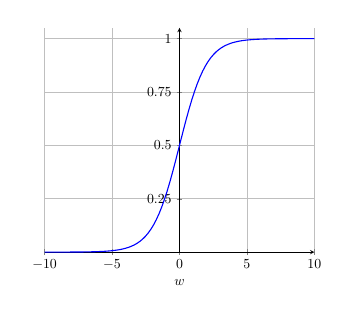
\begin{tikzpicture}[scale=0.5]
            \begin{axis}%
              [ %%%%%%%%%%%%%%%%%
              grid=major, %
              xmin=-10, % 
              xmax=10, % 
              axis x line=bottom, % 
              ytick={0,.25,.5,.75,1.0}, %
              ymax=1.05, % 
              axis y line=middle, % 
              xlabel = $\scal{\seq{w}}{\x}$, %
              %ylabel = $$, % 
              every  axis y label/.style={at={(current axis.north  west)},above=2mm} ]% 
              %%%%%%%%% binary classif in green
              \addplot%
              [ blue,thick,%
              mark=none, samples=100, domain=-10:10, ]
              (x,{1/(1+exp(-x))});
            \end{axis}
          \end{tikzpicture}
        \end{center}
        \end{minipage}
    \end{column}
  \end{columns}
\end{frame}

%%%%%%%%%%%%%%%%%%%%%%%%%%%%%%%%%%%%%%%%%%%%%%%%%%%%%%%%%%%%%%%%
\begin{frame}
  \frametitle{Logistic regression}

  The class $\class$ is the outcome of the binary random variable $\rvclass$
  \begin{block}{The sigmoid/logistic function}
    \begin{align*}
      y = P(\rvclass=1 | \x) &= \sigma(w_0 + \scal{\vct{w}}{\x}) \\
      \sigma(a)  &= \frac{e^a}{1+e^a} = \frac{1}{1+e^{-a}}\\
      a&=w_0 + \scal{\vct{w}}{\x} \in \mathbb{R}
    \end{align*}
  \end{block}
  \begin{center}
    \includegraphics[width=0.4\textwidth]{./figs/student_linear_1.pdf}
    \includegraphics[width=0.4\textwidth]{./figs/sigmoid_2d}
  \end{center}
\end{frame}

\begin{frame}{Logistic regression model for binary classification}
  \begin{itemize}
  \item The model is defined by $$ \params = (w_0 , \vct{w})$$
  \item Its output is $y = P(\rvclass=1|\x) = \sigma(w_0 + \scal{\vct{w}}{\x})$
  \item The decision rule ($\class$ inference from the model output $y$):
    \begin{align*}
      c=1 &\textrm{ if } y = P(\rvclass=1|\x) > P(\class=0|\x), &\textrm{ and } c=0 \textrm{ otherwise}\\
      c=1 &\textrm{ if } y = P(\rvclass=1|\x) > 0.5, &\textrm{ and } c=0 \textrm{ otherwise}
    \end{align*}
\end{itemize}
\begin{center}
Now let us define a criterion to \textit{learn} $\params$
\end{center}
\end{frame}



